\section{Atacs de descobriment d’informació del broker MQTT}

En aquest apartat es descriuen diferents atacs que permeten descobrir diferent informació interessant per a l'atacant explotant vulnerabilitats del broker MQTT. Per a realitzar aquests atacs, s'ha suposat coneguda l'adreça IP i port del broker MQTT així com altres dades que poden ser trobades mitjançant els atacs utilitzats en l'apartat anterior (\ref{sec:Recon}).


\subsection{Atacs de descobriment de credencials}

Una de les mesures de seguretat més comunes per als brokers MQTT és l'autenticació mitjançant nom d'usuari i contrasenya. Mosquitto, d'igual manera que la majoria de brokers MQTT comercials disposa d'un sistema per a generar fitxers de credencials d'usuari. Per a la realització d'aquest atac, he configurat el broker solament permetent l'entrada de l'usuari "tfg" amb la contrasenya "1234" amb mosquitto-passwd. Aquest genera un fitxer passwd on es guarda usuari:contrasenya amb la contrasenya encriptada amb bcrypt. \cite{bcryptexp}. Per altra banda, he generat un fitxer anomenat acl que genera una Access Control List que habilita o no a subscriure's (read) o publicar (write) a un tòpic específic (en aquest cas tfg/\#). El seu format és el següent:

\begin{lstlisting}[language=bash, caption={Access Control List}, label=lst:ACL]
user tfg
topic readwrite tfg/#
\end{lstlisting}

Per a descobrir credencials, s'ha elaborat un atac de força bruta mitjançant MQTT-SA (\ref{sec:MQTTSA}), una eina especialitzada en el protocol MQTT que permeten mitjançant llistes dels usuaris i credencials comprovar una gran quantitat de combinacions per tal d'accedir al broker i recopilar la validesa d'aquestes en un fitxer de sortida. Un exemple d'execució és:

\begin{lstlisting}[language=bash, caption={Execució de MQTT-SA}, label=lst:MQTTSAExec]
 python3 mqttsa.py -u "tfg" -w ./psw.txt -t 5 -mp 255 -mq 1000 192.168.0.40
\end{lstlisting}

\begin{figure}[H]
    \centering
    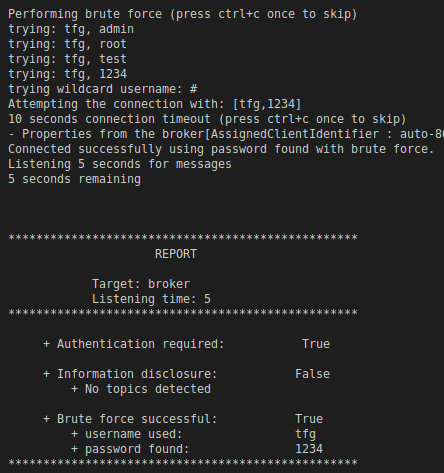
\includegraphics[width=0.7\textwidth]{img/mqttsa.png}
    \caption{Sortida de l'atac de força bruta amb MQTT-SA. S'observa com s'ha trobat l'usuari "tfg" amb la contrasenya "1234" adequadament. Apareix la IP amb el nom de "broker" degut a l'utilització de DHCP dintre els l'entorn de contneidors.}
    \label{fig:MqttsaBruteforce}
\end{figure}

\subsection{Subscripció a tòpics d'administració}

Una característica dels brokers MQTT, és l'ús de tòpics d'administració anomenats \textbf{\$SYS} que permeten als clients obtenir informació sensible sobre l'estat del broker i dels clients.

Per a la realització d'aquest atac, s'ha utilitzat un script de NMAP anomenat mqtt-subscribe que recopila tota aquesta informació subscrivint-se a tots els tòpics d'administració possibles. 
Una execució d'aquest atac per a un broker amb IP 192.168.0.40 és la següent:

\begin{lstlisting}[language=bash, caption={NSE script Nmap}, label=lst:NmapScript]
    nmap -Pn --script mqtt-subscribe -p 1883 -oG info_broker.txt 192.168.0.40
\end{lstlisting}

Amb aquest atac a un broker mosquitto com l'utilitzat en aquest treball, s'obté informació com ara:

\begin{itemize}
    \item Informació de la versió del broker i configuració general del broker.
    \item Nom d'usuari, estat de la connexió i keep alive dels clients.
    \item Nombre màxim de clients simultanis amb els quals pot treballar el broker.
    \item Mètriques de rendiment: bits enviats per segon, bits rebuts per segon, latència, etc
    \item Estadístiques de missatges enviats i rebuts.
    \item Llista de tòpics publicats i subscrits.
    \item Diversos errors i advertències del broker.
\end{itemize}

En aquest atac, el kali linux l'atacant genera un gran nombre de paquets MQTT subscribe per a subscrire's a aquests tòpics. 

\begin{figure}[H]
    \centering
    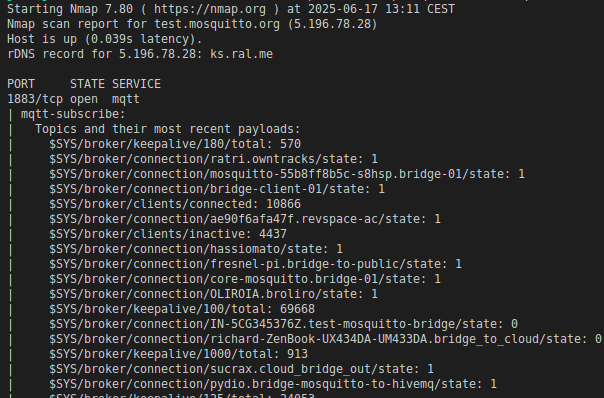
\includegraphics[width=0.7\textwidth]{img/nmapNSE.png}
    \caption{Petita part de la sortida de l'execució del script Nse "mqtt-subscribe".}
    \label{fig:NmapNSE}
\end{figure}

